% Nome do capítulo
\chapter{Proposta Técnica}
% Label para referenciar
\label{cap:4}
% Diminuir espaçamento entre título e texto
\vspace{-1.9cm}

Neste capítulo serão descritas a metodologia, o ambiente de testes e as tecnologias usadas no desenvolvimento do trabalho.

\section{Metodologia}
\label{sec:4:1}

Nesta seção será descrita a metodologia necessária para o desenvolvimento do trabalho.

\subsection{Levantamento Bibliográfica}
\label{sec:4:1:1}

Nessa etapa foi feita um levantamento bibliográfico. O objetivo é entender como funciona na teoria e na prática os algoritmos de localização e classificação de objetos. Além disso, o levantamento também serviu para definir a base de dados a ser utilizada no trabalho, a arquitetura de redes neurais convolutivas a ser implementada, a abordagem utilizada para fazer a localização e classificação de objetos e a métrica utilizada para avaliar o trabalho.

A arquitetura base selecionada foi a \ac{DenseNet}121, as bases de imagens selecionadas foram as versões de 2007 e 2012 da \ac{PASCAL VOC}. A abordagem selecionada para fazer a localização e classificação envolve elementos da \ac{SSD} \cite{wei-2015} e da \ac{DSSD} \cite{cheng-2017}. Por fim, a métrica utilizada é a \ac{mAP} conforme definida na Seção \ref{section:3:4:2}.

\subsection{Implementação e treinamento}
\label{sec:4:1:2}

Nesta fase foi feita a implementação da \ac{DenseNet}121 com as modificações propostas por \citeonline{wei-2015} e \citeonline{cheng-2017} para fazer a localização e classificação dos objetos. Feita a implementação da \ac{DenseNet} e das modificações, o modelo foi treinado usando a base de dados \ac{PASCAL VOC} nas versões 2007 e 2012. Mais detalhes das modificações feitas na arquitetura e do treinamento podem ser encontradas na Seção \ref{sec:4:3}.

\subsection{Testes e Avaliação}
\label{sec:4:1:3}

Nesta fase foram feitos os testes com o modelo proposto. Eles foram feitos usando o subconjunto de testes da \ac{PASCAL VOC} 2012. Após os testes, foi feita a avaliação dos resultados do modelo com a métrica proposta (\ac{mAP}). Em cima dos resultados obtidos foi feita uma comparação com os principais trabalhos relacionados na literatura \cite{wei-2015, cheng-2017} com o intuito de apontar as principais falhas e os principais ganhos do modelo proposto.

Além disso, foram feitas algumas demonstrações com o intuito de gerar imagens para se fazer uma avaliação qualitativa dos resultados obtidos pelo modelo. Por fim, foi escrita uma monografia contendo todo o conteúdo dos estudos realizados, das implementações feitas e dos resultados obtidos. O Capítulo \ref{cap:5} apresenta de forma mais detalhada os resultados obtidos nos experimentos feitos.

\section{Ambiente de teste}
\label{sec:4:2}

Todo o código foi implementado usando as seguintes tecnologias:

\begin{itemize}
	\item Python 3.5.2;
	\item TensorFlow 1.8.0;
	\item Keras 2.2.4;
	\item Jupyter 2.1.2;
	\item Notebook 6.0.3.
\end{itemize}

Os experimentos foram realizados no computador com as seguintes configurações:

\begin{itemize}
	\item \textbf{Sistema Operacional:} Ubuntu 18.04 LTS;
	\item \textbf{CPU:} Intel(R) Core(TM) i7-8700 CPU @ 3.20GHz (6 núcleos, duas \textit{threads} por núcleo);
	\item \textbf{Memória RAM:} 32GB;
	\item \textbf{GPU:} NVidia GTX 1080.
\end{itemize}

\section{Implementação e treinamento}
\label{sec:4:3}

Nesta seção será descrita de forma mais detalhada a implementação das modificações na arquitetura da rede neural, e o treinamento.


\subsection{Modificação da Arquitetura}
\label{secao:4:3:1}

A implementação consiste em adaptar a \ac{DenseNet} 121 para realizar as tarefas de localização e classificação. Nesse estágio foi feita uma pequena alteração com relação aos modelos propostos por \citeonline{wei-2015} e por \citeonline{cheng-2017}. Enquanto que \citeonline{wei-2015} usou imagens de tamanho $300 \times 300$ e \citeonline{cheng-2017} usou imagens de tamanho $321\times 321$, foi usado nesse trabalho imagens de $311 \times 311$.

O motivo é que, embora a \ac{DenseNet} possua as mesmas características de \textit{downsample} (por meio de convolução ou \textit{pooling}) que a \ac{ResNet}, a implementação da \ac{SSD} por \citeonline{cheng-2017} usa \textit{padding} válido para todas as camadas de \textit{downsample}. Isso faz com que, caso o tamanho de saída da camada de \textit{downsample} não seja inteiro, uma parte seja cortada, podendo causar perda de informação. Sendo assim, foi feita a opção por uma imagem com tamanho menor e o uso de \textit{padding} equivalente, de forma a evitar o corte.

Além dessas modificações, é necessário mudar algumas coisas na arquitetura da rede \ac{DenseNet}121. A primeira delas é que a SSD utiliza ramificações de diferentes níveis para fazer as predições de forma mais precisa. Sendo assim, a primeira alteração é que no segundo bloco de transição é criada uma ramificação fazendo regularização L2. Além disso, a camada de \textit{pooling} do último bloco de transição é substituída por um bloco $3\times3$ com strides igual a 1. No final da rede as camadas de \textit{pooling} global e softmax são removidas e essa saída é a segunda ramificação da \ac{SSD}. Depois disso, são adicionados mais dois blocos com camadas de convolução, uma $1\times1$ seguida de um $3\times3$ com \textit{stride} 2. Por fim, mais dois blocos, com as mesmas camadas, porém, as camadas $3\times3$ com \textit{stride} igual a 1. A Figura \ref{fig:dense_ssd} mostra a nova arquitetura da rede. Os blocos brancos representam as partes da implementação original da \ac{DenseNet}121, os blocos azuis representam as modificações propostas por \citeonline{wei-2015} e os blocos laranjados representam as modificações propostas por \citeonline{cheng-2017}.

\begin{figure}[H]
	% Alterar espaçamentos antes e depois do caption
	\setlength{\abovecaptionskip}{0pt}
	\setlength{\belowcaptionskip}{0pt}
	% Caption
	\caption[Arquitetura proposta]{Arquitetura com modificações propostas para a \ac{DenseNet}}
	\centering
	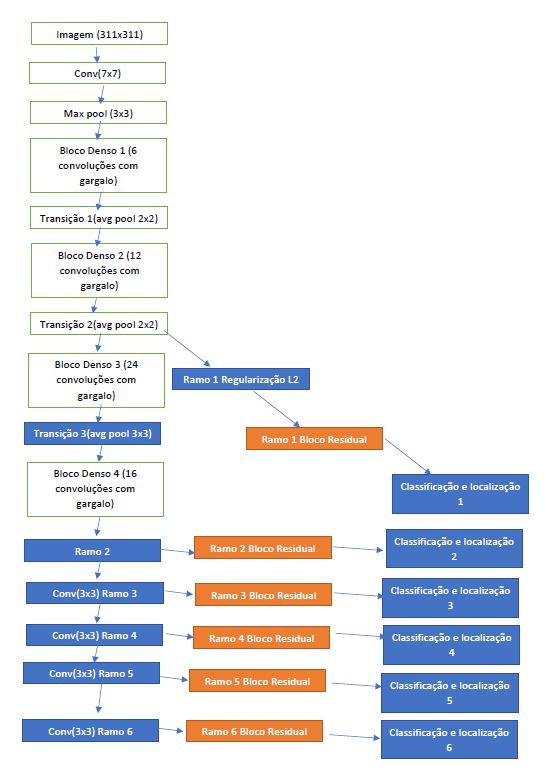
\includegraphics[width=.6\textwidth]{imagem/0x_densenet_classloc.jpg}
	% Caption centralizada
	\captionsetup{justification=centering}
	\captionfont{\small{\textbf{\\Fonte: Elaborado pelo autor.}}}	
	\label{fig:dense_ssd}
\end{figure}


\subsection{Treinamento}
\label{secao:4:3:2}

A rede foi inicializada com os pesos da \ac{DenseNet}121 treinada na ImageNet, e as camadas adicionais foram inicializadas com o método \textit{He normal} proposto por \citeonline{he-2015}. O algoritmo de treinamento selecionado foi o Adam, proposto por \citeonline{kingma-2014} com os seguintes hiperparâmetros:

\begin{itemize}
	\item $\alpha = 5\times10^{-5}$;
	\item $\beta_1 = 0,9$;
	\item $\beta_2 = 0,999$;
	\item $\epsilon = 1\times10^{-8}$.
\end{itemize}

Além disso, o treinamento ocorreu em um total de 400 épocas, cada época com 1000 iterações e cada iteração com um lote de processamento de 12 imagens. Após 200 épocas de treinamento, a taxa de aprendizado caiu para $5\times10^{-6}$ e após mais 100 épocas, caiu para $5\times10^{-7}$. As bases de dados usadas para os testes foram a \ac{PASCAL VOC} 2007 e 2012. Para treinamento foram usadas as imagens do conjunto de treino e validação de ambas as bases, e para validação do treinamento foi utilizada a base de testes de 2007. Os testes foram feitos na base de 2012.